\section{CUDA Memory Architecture}
\label{sec:cuda memory architecture}

This section aims to give a brief overview of the memory architecture of CUDA-enabled GPUs.

\Cref{fig:cpu gpu communication} illustrates the connections between the different layers of memory.
Starting from the bottom, we have the mapped memory from the host machine to global memory on the GPU device.
The global memory of the device is the slowest on the device.
As the memory moves towards the cores, access to the memory is much faster.

\begin{figure}[htb]
  \centering
  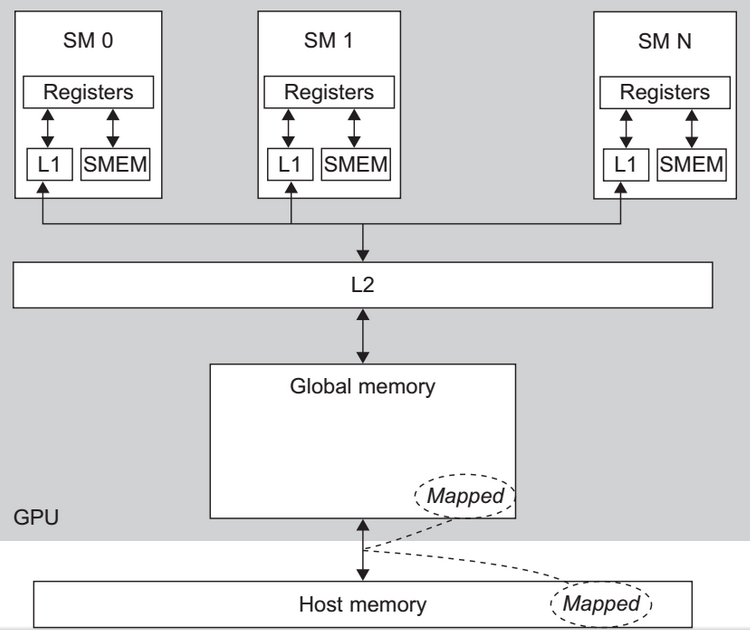
\includegraphics[height=7.5cm]{graphics/images/cuda-mem-hierarchy.png}
  \caption{CUDA memory hierarchy~\cite{farber2011cuda}}
  \label{fig:cpu gpu communication}
\end{figure}

The L2 cache fetches data in a Least Recently Used (LRU) fashion, which means that it is built for temporal locality, i.e. recently accessed data is assumed to likely be used again in the near future.
\todo{is shared memory bandwidth the same for L1, L2, and SMEM?}
The L1 cache is designed for spacial locality, i.e. adjacent memory locations to the wanted data is also cached, with the assumption that neighbouring data will be used in the near future.
This means that the memory that is inside the SM is best suited for coalesced memory access (see \cref{sec:coalesced}).


\begin{table}[htb]
  \centering
  \begin{tabular}{l r}
    \toprule
    memory & speed \\
    \midrule
    register & $\approx \SI{8000}{GB/s}$ \\
    shared   & $\approx \SI{1600}{GB/s}$ \\
    global   & $\SI{177}{GB/s}$ \\
    mapped   & $\approx \SI{8}{GB/s}$ \\
  \end{tabular}
  \caption{GPU memory bandwidth~\cite{farber2011cuda}}
  \label{tab:hardware connections transfer rates}
\end{table}

\Cref{tab:hardware connections transfer rates} summarises the transfer rates of different connections of the different types of memory connections.
